\section{RTDroid - Versione base}
RTDroid si pone l'obiettivo di aggiungere supporto real-time ad Android nella sua interezza. Questo significa che tutti i problemi sopra riportati devono essere corretti in modo da fornire un supporto completo e che dia garanzie solide. In questa estensione, solamente un processo di livello utente (l'applicazione) è in esecuzione. 

Per risolvere tutti i problemi di Android è necessario un redesign profondo che arriva fino al livello del kernel. Quest'ultimo viene sostituito con un kernel real-rime, LinuxRT o, meglio, RTEMS. Anche la VM di Android viene sostituita, con Fiji. Sopra questo nuovo strato vengono offerte le ''classiche'' API Android, con l'aggiunta di una serie di estensioni che correggono specifici problemi riscontrati. Queste API aggiuntive rispettano la RTSJ. 

\subsection{Looper e Handler}
Ad ogni messaggio viene assegnata una priorità, attraverso due modalità:
\begin{itemize}
	\item\textit{inheritance}: il messaggio eredita la priorità del mittente;
	\item\textit{inheritance + specified}: il mittente può specificare una priorità relativa a tutti i messaggi inviati.
\end{itemize}
Dopodiché viene definita una coda per ogni priorità, con associati un \texttt{Looper} e un \texttt{Handler}. Messaggi a priorità più bassa non ritarderanno quelli a priorità più alta. Per avere garanzie sulla quantità di memoria utilizzata, le code possono essere dimensionate staticamente.

\subsection{AlarmManager}
Sia la registrazione che la consegna devono essere ridefinite per un completo supporto real-time. Per la registrazione vengono utilizzati degli alberi rosso neri (Figura~\ref{fig:rtalarm}), così da rendere il processo prevedibile sulla base della complessità delle operazioni sull'albero. 
\begin{figure}[h]
	\centering
	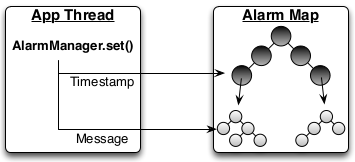
\includegraphics[width=0.6\linewidth]{rtalarm}
	\caption{Registrazione di allarmi real-time}
	\label{fig:rtalarm}
\end{figure}

L'albero principale mantiene i timestamp delle registrazioni e dei puntatori ad altri alberi, che ordinano i timestamp sulla base della priorità del richiedente. Di conseguenza una registrazione include solamente due inserimenti. Organizzando gli alberi in base alla priorità si ha la garanzia che un messaggio diretto ad un thread a bassa priorità non ritardi uno a priorità più alta. In questo modo, anche se un thread a bassa priorità registra un sacco di eventi (più di quanti ne possono essere gestiti), i thread a priorità più alta non verranno in nessun modo toccati.

Per la consegna viene definito un \texttt{AlarmManager} thread a cui è assegnata la priorità più alta di tutte. Questo thread sostituisce il classico meccanismo di invio di messaggi di Android. Si sveglia ogni volta che c'è un inserimento in un albero rosso nero e pianifica un thread all'istante temporale specificato. A quest'ultimo viene associata la callback specificata dall'applicazione.

\subsection{SensorManager}
Il sensing funziona attraverso un \textit{polling thread} che periodicamente ascolta l'ambiente circostante. Questo comunica con vari \textit{processing thread}, uno per ogni sensore, che interpretano i dati ricevuti dal polling thread.

I problemi riportati vengono risolti attraverso \textit{priority inheritance}. Quando un thread con priorità \texttt{p} registra un listener per un sensore, al thread associato a quel sensore viene assegnata la priorità \texttt{p}. Se più di un thread si associano allo stesso sensore, allora al thread del sensore è associata la priorità più alta tra tutti. Anche i thread creati per eseguire le callback hanno assegnata la priorità \texttt{p}. Il polling thread ha la priorità più alta di tutte, in modo da assicurare che i dati vengano raccolti appena possibile.

Quando un'applicazione registra un nuovo listener per un sensore viene di fatto creato un nuovo percorso di consegna dal polling thread al listener. Questo percorso è isolato ed eredita la priorità del thread che l'ha creato. 

\subsection{Sostituire componenti non real-time con componenti real-time}
Il kernel Linux di Android ha molte modifiche per renderlo adatto all'utilizzo in un ambiente con risorse limitate. Questo diventa un problema quando si cerca di sostituire alcuni componenti per migliorare il supporto real-time.

\paragraph{Bionic.} Un esempio è dato dalle librerie C native. Al posto di \texttt{glibc} Android utilizza \textit{Bionic}. Bionic è una libreria C leggera e altamente semplificata ed ottimizzata in modo da poter essere utilizzata in ambienti con risolrse limitate, in particolare CPU a bassa frequenza e poca memoria. Tra le funzionalità eliminate c'è la gestione delle eccezioni C++, che provoca un grandissimo overhead in \texttt{glibc}. Questa esclusione non è però problematica, dato che Android si basa su Java, e dunque le eccezioni sono gestite più ad alto livello, tramite Java. Sfortunatamente però non aderisce alla specifica POSIX e non supporta le estensioni real-time di mutex e pthreads. Una modifica di questa libreria è necessaria per utilizzare una VM real-time, come Fiji.

\paragraph{Patch del kernel incompatibili.} Android ha introdotto molte modifiche al kernel Linux, tanto che l'applicazione automatica di patch per ottenere RTLinux è impossibile, e deve essere fatta manualmente. Anche dopo averla fatta manualmente, comunque, il kernel rimane non completamente prerilasciabile e questo comporta alti tempi di attesa possibili. 

\paragraph{Funzionalità non real-time del kernel.} Il kernel Android ha due funzionalità critiche sotto l'aspetto real-time. La prima è l'\textit{out of memory killer} (OOM), che viene avviato in condizioni di bassa memoria disponibile. Analizza tutte le pagine di memoria per verificare che il sistema sia veramente in condizioni critiche ed uccide un processo selezionato. I thread in esecuzione vengono fermati e bloccati per un periodo di tempo variabile. In un contesto dove è permessa solo l'esecuzione di un processo utente, però, OOM è inutile.

Un'altra funzionalità problematica è CPUFreq, che scala dinamicamente la frequenza della CPU. Android la usa per bilanciare le performance e la l'utilizzo della batteria. Il problema è che, quando CPUFreq cambia la frequenza, il cambiamento è percepito da tutti i thread running, introducendo jitter nel sistema. Inoltre il cambiamento non è tenuto in considerazione quando viene fatto lo scheduling, e quindi ci potrebbero essere deadline mancate e picchi di latenza non previsti. Esistono, comunque, scheduling real-time che tengono in considerazione i cambiamenti di voltaggio, e questi sono applicabili in questo contesto. Attualmente non ci sono soluzioni, ma una possibilità è considerare il caso peggiore (tutti i task nel loro caso peggiore e la peggiore frequenza possibile), anche se questo non considera il jitter del cambiamento di frequenza.

\section{RTDroid Migliorata}
La principale limitazione dell'approccio precedente è che viene data la possibilità di eseguire solo un processo utente per volta. Una seconda versione di RTDroid mira a risolvere questo problema, supportando l'esecuzione di più applicazioni real-time e non, come mostrato in Figura~\ref{fig:rtdroid}.

\begin{figure}[h]
	\centering
	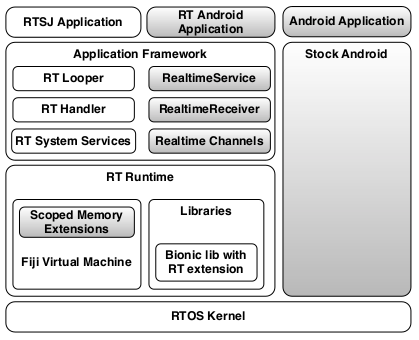
\includegraphics[width=0.6\linewidth]{rtdroid}
	\caption{RTDroid}
	\label{fig:rtdroid}
\end{figure}

Oltre ai cambiamenti introdotti precedentemente, RTDroid aggiunge costrutti real-time di alto livello, come (\textit{RealtimeService} e \textit{RealtimeReceiver}), costrutti di basso livello per la comunicazione (\textit{Realtime Channels}) e un meccanismo per specificare proprietà di questi costrutti. Le applicazioni senza vincoli temporali vengono eseguite in una VM separata. Questa modalità è utile anche per i componenti grafici delle applicazioni real-time. Figura~\ref{fig:rtbootstrap} mostra il bootstrap.
\begin{figure}[h]
	\centering
	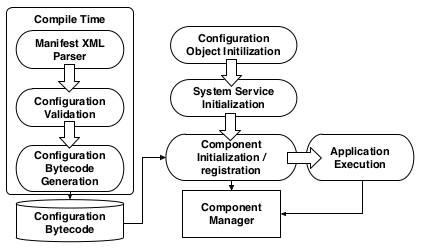
\includegraphics[width=0.6\linewidth]{rtbootstrap}
	\caption{Bootstrap di RTDroid}
	\label{fig:rtbootstrap}
\end{figure}

Quest'ultimo è divisa in compile time e runtime. Il processo a due fasi assicura che la memoria possa essere pre allocata e che i componenti siano correttamente configurati. Durante la compilazione viene fatto il parsing del manifest, vengono eseguiti dei controlli e viene generato il bytecode per la configurazione di tutti i componenti coinvolti. Questo bytecode rappresenta un gestore per ogni componente dell'applicazione. All'avvio, il sistema analizza la lista dei gestori e chiama quello appropriato per istanziare il componente corrispondente. Dopo l'istanziazione, il componente viene registrato presso un \textit{Component Manager}, che ne gestisce il ciclo di vita.

\subsection{Componenti}
RTDroid supporta tre diversi componenti real-time: \textit{services}, \textit{tasks} e \textit{receivers}. Un \texttt{RealtimeService} corrisponde ad un normale service Android, utilizzato per compiti aperiodici o sporadici. Dato che la nozione di computazione periodica non è presente in Android, viene introdotta la classe \texttt{PeriodicTask} per modellarla. \texttt{RealtimeReveiver}, invece, è usato per reagire ad eventi consegnati attraverso \texttt{Intent}. Non c'è bisogno di fornire un corrispettivo delle Activity. Queste ultime vengono utilizzate per la programmazione delle UI e possono essere eseguite senza vincoli temporali. L'interazione tra componenti real-time e non (UI) è permessa.

Ai componenti real-time viene assegnata una priorità, un tempo di inizio, una deadline e un limite di memoria. Questo viene fatto staticamente, estendendo i tag utilizzabili nel manifest.

Gestire il ciclo di vita dei componenti significa: 
\begin{enumerate}
	\item assicurare che priorità, deadline e periodicità vengano rispettate;
	\item gestire automaticamente la memoria allocata;
	\item garantire che i limiti per ogni componente siano rispettati.
\end{enumerate}
Per (2) viene utilizzata un'allocazione basata sulle regioni. L'idea è di non gestire oggetti singoli, ma di allocare gli oggetti in regioni e poi operare al livello di una regione. L'idea è stata introdotta da RTSJ con le aree di memoria \textit{scoped}. I benefici principali sono due: i thread non devono essere bloccati durante la GC ed è possibile limitare il numero di regioni allocate da ciascun thread.

RTDroid supporta una forma semplificata di memoria scoped. Ogni componente ha accesso a due scope: \textit{Persistent Memory}, per dati la cui vita è legata al componente, e \textit{Release Memory}, che viene pulita prima di ogni rilascio di un componente periodico. La dimensione di queste aree è definita nel manifest. La memoria totale assegnata ad un componente è la somma di peristent memory, release memory e memoria assegnata ai sotto-componenti.

\paragraph{Service} \mbox{} \\
Un service real-time è una classe astratta e un programmatore deve implementare le sue callback. Queste sono ereditate direttamente da \texttt{Service} di Android e vengono invocate nei diversi stadi del ciclo di vita. Contrariamente ad Android, che esegue i service nello stesso thread della UI, RTDroid li esegue in thread separati (mappati con i thread real-time della JVM sottostante), in modo da supportare diverse priorità. Quando viene inizializzato, ad un service viene assegnata una persistent memory che ha lo stesso tempo di vita del service stesso (allocata allo start e deallocata alla terminazione). Inoltre, se vengono utilizzati dei canali di comunicazione, le code per gli intent sono allocate nella persistent memory. Oltre ai task periodici, anche le callback eseguono utilizzando la release memory, che viene pulita al termine dell'esecuzione. La struttura è mostrata in Figura~\ref{fig:scopeservice}.

Il manifest deve dichiarare quanta memoria è richiesta, in modo da dimensionare in modo corretto.
\begin{figure}[h]
	\centering
	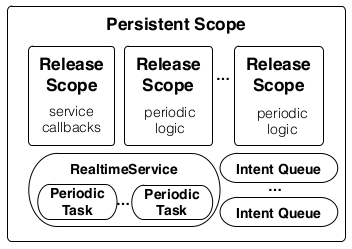
\includegraphics[width=0.6\linewidth]{scopeService}
	\caption{Struttura dello scope per un Service}
	\label{fig:scopeservice}
\end{figure}

\paragraph{Task periodici}\mbox{} \\
Un task periodico è un sotto-componente di un service. Oltre alle caratteristiche del parent, un task ha bisogno di un periodo.

\paragraph{Receiver}\mbox{} \\
In Android, un nuovo broadcast receiver viene allocato ogni volta che un intent è ricevuto. Se tanti intent vengono inviati ad un componente, il risultato è una frequente allocazione/deallocazione. In RTDroid, invece, un receiver real-time è un costrutto persistente, e viene riutilizzato per ridurre l'impatto sulla memoria. Come conseguenza diretta,un receiver può processare un solo intent alla volta, e la logica dell'applicazione è espressa a callback. In \texttt{onReceive()} va specificato come si reagisce aglie eventi, mentre \texttt{onClean()} è usato per pulire la memoria. La sua implementazione è necessaria se si desidera avere una gestione stateless degli eventi, ed è non necessaria se vengono modificate solo variabili locali che risiedono nella release memory, che viene pulita automaticamente.

Un'importante scelta progettuale riguarda la priorità delle callback. Queste vengono eseguite alla stessa priorità dei loro componenti. Callback multiple generate da una serie di intent sono eseguite in ordine. Dal punto di vista implementativo eusto significa che un receiver è collegato ad un gestore di eventi asincrono nella JVM, che gestisce le ricezioni con una coda a priorità. Questo assicura che messaggi provenienti da mittenti ad alta priorità verranno consegnati prima. 

\subsection{Comunicazione}
RTDroid fornisce quattro tipi di canali real-time:
\begin{itemize}
	\item message;
	\item broadcast;
	\item trasferimento di grandi quantità di dati;
	\item cross-context, per comunicare ocn componenti non real-time.
\end{itemize}
I programmatori devono specificare il nome del canale, il tipo di dato trasferito e la sua dimensione. Inoltre, i componenti real-time devono specificare il numero di messaggi che invieranno e riceveranno nel corso della loro vita. Questo assicura la possibilità di preallocare gli oggetti corrispondenti ai messaggi e di tenere sotto controllo i limiti di memoria per ciascun componente. Di questi quattro canali, i primi tre devono esplicitamente essere creati dai programmatori, mentre ne esiste uno predefinito per la comunicazione con i componenti non real-time.

Ogni canale deve specificare (nel manifest) il suo comportamento a runtime come segue: tipo, ordine di ricezione dei messaggi, priorità dell'esecuzione della callback associata e politica di cancellazione, tipo e dimensione dei dati. I compoennti possono utilizzare \texttt{intent-filter} per identificarsi come publishers o subscribers e specificare il numero di messaggi letti o inviati in ogni rilascio della callback. 

Il principale beneficio dell'utilizzo del manifest è che c'è un controllo statico. RTDroid garantisce la correttezza dell'applicazione in due aspetti:
\begin{itemize}
	\item check dei limiti di memoria: la memoria richiesta da un componente deve essere uguale alla somma di persistent, release e memoria dei sotto-componenti;
	\item check di channel overflow: il tasso di messaggi in entrata non dovrebbe eccedere il limite dei messaggi processabili da quel canale.
\end{itemize}

\paragraph{Message channels} \mbox{} \\
Un canale di questo tipo ha tre caratteristiche principali:
\begin{enumerate}
	\item il \texttt{RealtimeHandler} associato deve essere registrato un un service real-time;
	\item possono essere scambiati solo array di tipi primitivi o buffer di byte a lunghezza fissa;
	\item il numero di messaggi in attesa è limitato.
\end{enumerate}

RTDroid crea una coda a dimensione fissa per ogni canale. Anche i messaggi sono preallocati, e vivono nella persistent memory del destinatario. Figura~\ref{fig:messagechannel} mostra la gerarchia nella memoria scoped.
\begin{figure}[h]
	\centering
	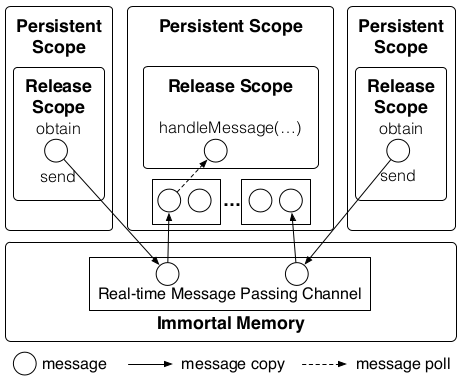
\includegraphics[width=0.6\linewidth]{messageChannel}
	\caption{Real-time message channels}
	\label{fig:messagechannel}
\end{figure}

L'accodamento dei messaggi è gestito alla priorità del mittente, mentre l'estrazione è gestita alla priorità del destinatario. Se la coda è piena, un componente ad alta priorità può rubare un messaggio ad un mittente con bassa priorità. Quando questo accade, il componente ad alta priorità sarà in grado di accodare il messaggio, mentre quello a bassa priorità riceverà un'eccezione.

L'invio è difficoltoso perché i messaggi sono preallocati e i mittenti non dovrebbero mantenere riferimenti ai messagi dopo che questi sono stati inviati. Il protocollo usato è quindi indiretto. Una \texttt{MessageClosure} è allocata dal mittente, e la callback \texttt{getMsg()} è usata per popolare il payload.

Il riferimento al messaggio viene dato in base alla priorità del mittente. Di conseguenza l'operazione può fallire se non ci sono messaggi con quella priorità (sono tutti in uso). In questo caso viene lanciata un'eccezione. Se un componente ad alta priorità cerca di ottenere un messaggio, ma sono tutti utilizzati, può rubare un messaggio correntemente in uso da un componente non real-time a priorità più bassa. Dato che tutti i messaggi sono ottenuti durante il metodo \texttt{send} di \texttt{MessageClosure}, tutti i messaggi in uso corrispondono a messaggi accodati, ma non ricevuti. Se il messaggio viene rubato viene sollevata un'eccezione asincrona, utilizzando il meccanismo \texttt{AsynchronousInterruptedException} previsto da RTSJ.

Una volta che un messaggio viene ottenuto, il mittente deve copiare i dati da inviare dal suo spazio di memoria allo spazio del canale. Questo assicura che un mittente non possa utilizzare o riempire lo spazio del destinatario direttamente, ma è quest'ultimo a dover accettare la ricezione. Una volta che il messaggio è copiato dall'handler del destinatario, l'oggetto del messaggio è rimesso nel pool. Questa strategia mantiene costante l'ammontare di memoria dedicata al passaggio dei messaggi. Il mittente deve utilizzare la sua memoria per memorizzare i dati che vuole inviare e non può usare le risorse del sistema finché non gli viene concesso il messaggio.

\paragraph{Broadcast Channel} \mbox{} \\
Questi canali sono usati per invocare callback in componenti real-time, disaccoppiando la priorità della consegna dell'intent dall'invocazione delle callback. La differenza tra messaggi e intent è che i primi hanno un solo destinatario, mentre i secondi no e per riceverli bisogna esplicitarlo nel manifest. 

\begin{figure}[h]
	\centering
	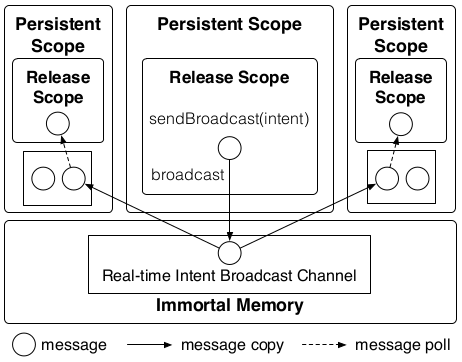
\includegraphics[width=0.6\linewidth]{images/broadcastChannel}
	\caption{Real-time broadcast channels}
	\label{fig:broadcastchannel}
\end{figure}

Figura~\ref{fig:broadcastchannel} mostra come un intent persiste nella memoria immortal fino a quando non è copiato in tutte le code dei subscribers. Sebbene il messaggio sia replicato per ogni subscriber, solo una copia è salvata nel canale. Il numero di destinatari è salvato in un contatore, e viene decrementato ad ogni ricezione. L'ultimo destinatario rilascia il messaggio e lo rimette nel pool, esattamente come nei message channels. L'utilizzo di memoria è limitato.

\paragraph{Bulk Data Channels} \mbox{} \\
Questo canale permette di trasferire dati di grandi dimensioni senza copiarli. Per supportarli viene esteso il concetto di memoria annidata con quello di memoria annidata trasferibile. Uno scope, che incapsula i dati, vene rimosso dallo stack del mittente e messo nello stack del destinatario. Di conseguenza, il mittente non può né allocare né scrivere dati in quello scope. L'idea funziona solo se il frame è il primo nello stack e se lo stack è lineare. Dato che gli scopes non sono esposti ai programmatori, i vincoli sono rispettati per costruzione dalla struttura del canale. In parole povere, quindi, questi canali permettono al mittente di creare uno scope trasferibile, di popolarlo con i dati, e di cederne l'accesso.

\paragraph{Cross-Context Channels} \mbox{} \\
Questi canali permettono alle Activities di comunicare con i componenti real-time. La comunicazione avviene tra due diverse VM, una delle quali esegue codice non real-time e RTDroid, che esegue applicazioni real-time. In questo modo si può interagire sia con il sistema Android che con le altre applicazioni. Al fine di questa comunicazione un'applicazione deve dichiarare un service, \texttt{RTsProxyService}, che sottoscrive un canale dichiarato in un'applicazione real-time. Nell'altra direzione, un'applicazione real-time si deve solo sottoscrivere agli intent che l'applicazione non real-time ha dichiarato nel suo manifest. Il service proxy permette al codice non real-time di inviare messaggi ai componenti real-time. Per limitare la memoria il numero di intent in un canale è limitato e ogni intent ha un payload di lunghezza fissata.
\begin{figure}[h]
	\centering
	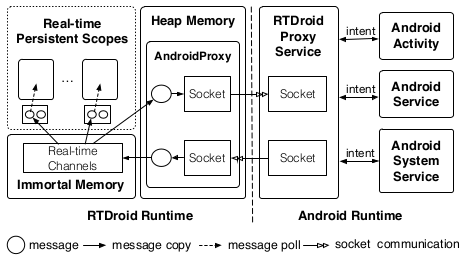
\includegraphics[width=0.6\linewidth]{crosscontentChannel}
	\caption{Cross-Content channel}
	\label{fig:crosscontentchannel}
\end{figure}

Figura~\ref{fig:crosscontentchannel} mostra come la comunicazione bidirezionale viene stabilita attraverso sockets. Vengono usati due componenti proxy in ogni runtime. Per evitare interferenza, il proxy di Android è eseguito sullo heap ed esegue ad una priorità real-time bassa. I messaggi in arrivo sono tradotti in intent o messaggi real-time con la più bassa priorità e inviati (attraverso canali real-time) ai componenti opportuni. In questi canali viene depositato solo un messaggio alla volta, in modo da evitare che componenti non real-time esauriscano la memoria usata da quelli real-time. I primi possono esaurire lo heap, ma questo non ha nessuna ripercussione sui secondi, che usano regioni preallocate.

\subsection{Gestione della memoria}
Fornire garanzie sulla memoria implica che il sistema sottostante deve fornire un'allocazione prevedibile (cioè l'allocazione degli oggetti non deve essere bloccata dal fatto che qualcun altro sta usando la memoria) e una reclamazione prevedibile (la gestione della memoria non deve interferire con l'esecuzione di componenti real-time). Per entrambi si usa la scoped memory, che fornisce una quantità fissa di memoria per task real-time con allocazione e deallocazione prevedibili. In aggiunta, la memoria scoped assicura che i thread real-time non siano bloccati durante la GC (se usano solo scoped memory). Come già detto, la RTSJ prevede tre tipi di memoria: 
\begin{itemize}
	\item heap, che è garbage collected;
	\item immortal, mai reclamata;
	\item scoped, fornisce regioni di dimensione fissa.
\end{itemize}
Per garantire l'integrità dei riferimenti RTSJ impone un'insieme di regole sulla gestione della scoped memory, ad esempio:
\begin{itemize}
	\item gli oggetti in uno scope sono reclamati solo quando tutti i thread in quello scope sono terminati;
	\item ogni thread deve entrare in uno scope sempre dallo stesso parent scope;
	\item uno scope con un tempo di vita lungo non può mantenere un riferimento ad un oggetto allocato in uno scope con un periodo di vita più corto. 
\end{itemize}

Le esecuzioni di componenti e callback (e le allocazioni associate) vengono separate per fornire un limite alla memoria occupata da ciascun componente. Il ciclo di vita di un componente viene gestito nel persistent scope (persistent memory), mentre l'invocazione delle callbacks viene gestita nel release scope (release memory). Ogni componente è legato ad un thread di controllo che è avviato nell'immortal memory. Questo assicura che la memoria necessaria per creare il contesto di esecuzione sia sempre disponibile. La stessa cosa vale anche per i canali di comunicazione.

\subsection{Valutazione}
\subsubsection{Micro Benchmark dei canali}
Il test vede due servizi real-time (alta priorità) che si scambiano messaggi (un sender e un receiver) ogni 100ms e uno non real-time che genera rumore (bassa priorità). Quest'ultimo esegue nello heap e fa partire 30 thread che disturbano lo scambio di messaggi. Questi thread sono di tre tipi:
\begin{itemize}
	\item heap noise, allocano un array di 512 byte nello heap ogni 200ms;
	\item computational noise, calcolano $\pi$ ogni 200ms;
	\item message noise, inviano un messaggio a bassa priorità al service receiver ogni 200ms.
\end{itemize}

\begin{figure}[h]
	\centering
	\begin{subfigure}[b]{0.3\textwidth}
		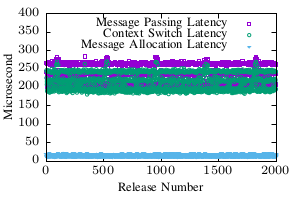
\includegraphics[width=\textwidth]{messagePassing}
		\caption{Scambio di messaggi}
		\label{fig:messagePassing}
	\end{subfigure}
	~ 
	\begin{subfigure}[b]{0.3\textwidth}
		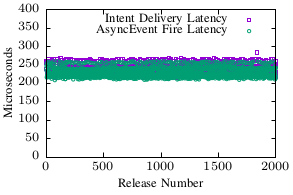
\includegraphics[width=\textwidth]{intentBroadcast}
		\caption{Intent broadcast}
		\label{fig:intentBroadcast}
	\end{subfigure}
	~
	\begin{subfigure}[b]{0.3\textwidth}
		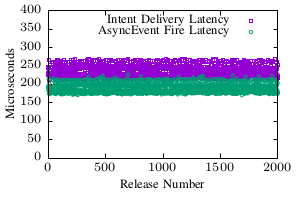
\includegraphics[width=\textwidth]{bulkData}
		\caption{Trasferimento di dati pesanti}
		\label{fig:bulkData}
	\end{subfigure}
	\caption{Baseline per la valutazione delle prestazioni dei canali}\label{fig:baselines}
\end{figure}

Figura~\ref{fig:baselines} mostra le misurazioni delle prestazioni senza interferenza. Lo scambio di messaggi consiste nell'allocazione del messaggio (da parte del mittente), nella sua consegna e nel context switch mittente/destinatario. Figura~\ref{fig:messagePassing} mostra la situazione con solo mittente e destinatario. Viene mostrata la latenza per 2000 eventi generati dallo scambio dei messaggi. Per ogni evento si definisce:
\begin{itemize}
	\item \textbf{message allocation latency}: tempo necessario per istanziare un messaggio;
	\item \textbf{message passing latency}: tempo necessario per la consegna;
	\item \textbf{context switch latency}: tempo trascorso tra l'invio del messaggio e il momento in cui questo viene processato.
\end{itemize}
I tre tipi di latenza sono strettamente limitati per tutti gli eventi, senza nessun punto anomalo che si discosta fortemente dagli altri. Senza nessun sovraccarico, questa architettura è stabile e prevedibile.

Un esperimento simile viene fatto con gli intents. Il mittente invia un intent ogni 100ms, e il receiver esegue una callback che, semplicemente, risponde al messaggio. Si definiscono:
\begin{itemize}
	\item \textbf{intent delivery latency}: latenza complessiva per ogni intent;
	\item \textbf{callback trigger latency}: tempo richiesto per generare una nuova callback.
\end{itemize}
I risultati sono mostrati in Figura~\ref{fig:intentBroadcast}, e sono simili a quelli precedenti.

Allo stesso modo, Figura~\ref{fig:bulkData} mostra la baseline per il trasferimento di dati di grosse dimensioni. La \textbf{transfer latency} è il tempo di consegna di un intent con un payload molto pesante.

\begin{figure}[h]
	\centering
	\begin{subfigure}[b]{0.3\textwidth}
		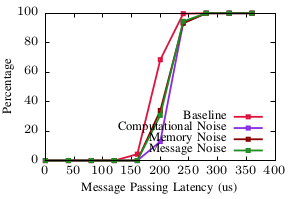
\includegraphics[width=\textwidth]{messagePassingLatency}
		\caption{CDF per lo scambio di messaggi}
		\label{fig:messagePassingLatency}
	\end{subfigure}
	~ 
	\begin{subfigure}[b]{0.3\textwidth}
		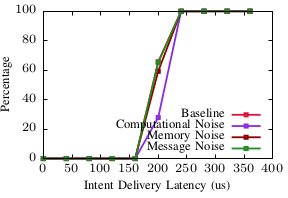
\includegraphics[width=\textwidth]{intentDeliveryLatency}
		\caption{CDF per il broadcast di Intent}
		\label{fig:intentDeliveryLatency}
	\end{subfigure}
	~
	\begin{subfigure}[b]{0.3\textwidth}
		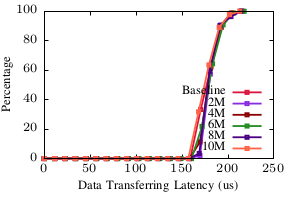
\includegraphics[width=\textwidth]{bulkdataLatency}
		\caption{CDF per il trasferimento di dati pesanti}
		\label{fig:bulkdatalatency}
	\end{subfigure}
	\caption{CDF delle prestazioni dei canali}\label{fig:cdfchannels}
\end{figure}

Figura~\ref{fig:cdfchannels} mostra i grafici CDF (cumulative distribution function) che confrontano le prestazioni dei tre tipi di canali. In particolare, i CDF illustrano che percentuale dei punti misurati è minore o uguale di un certo valore temporale. Per il messaging (Figura~\ref{fig:messagePassingLatency}), indipendentemente dal carico a cui è sottoposto, RTDroid si comporta bene (non ci sono grossi cambiamenti di latenza). Sebbene i risultati siano simili per gli intents (Figura~\ref{fig:intentDeliveryLatency}), si nota un overhead maggiore rispetto al messaging semplice. Questo era prevedibile, dato che l'intent è associato all'esecuzione di una callback. Figura~\ref{fig:bulkdatalatency} mostra i risultati per il trasferimento di dati di diverse dimensioni. RTDroid praticamente non risente del cambiamento di dimensioni (giustamente, perché non fa nessuna copia dei dati).

\subsection{Confronto con Android e con RTSJ}
Per confrontare RTDroid con Android e RTSJ vengono utilizzate tre applicazioni con vincoli temporali.
\paragraph{Cochlear Implant.}
Questa applicazione ha un service real-time per processare segnali audio e un receiver real-time per controllare che non ci siano errori nell'output. Ogni esecuzione del primo comporta l'acquisizione di 128 campioni, la loro elaborazione e il loro invio al receiver. Tutto questo non deve occupare più di 8ms. 

\paragraph{jPapaBench.} jPapaBench è un benchmark Java real-time che simula un software di controllo aereo. La versione utilizzata per la valutazione ha due services: un pilota automatico che esegue sensing, stabilizzazione e controlli vari e un fly-by-wire che gestisce i comandi radio e i controlli di sicurezza. La comunicazione originale è rimpiazzata con broadcast di intent. Il task di stabilizzazione ha una deadline di 50ms.

\paragraph{Wind Turbine Health Monitoring.} Questa applicazione è stata originariamente implementata utilizzando RTSJ. Dato che richiede hardware specializzato non è stata implementata in Android. Il suo compito è di rilevare rotture nelle turbine basandosi sui segnali acustici che emettono. Si compone di un task che emette un segnale audio, di uno che lo rileva e lo memorizza e di un terzo che rileva le rotture analizzando i segnali rilevati. La rilevazione deve avvenire ogni 50ms. In questo caso, la dimensione dei dati raccolti per ogni test sfiora i 2MB ed è quindi necessario sfruttare canali di comunicazione adatti. RTSJ, che non dispone dei canali di RTDroid, utilizza un buffer di memoria condiviso.

\begin{figure}[h]
	\centering
	\begin{subfigure}[b]{0.3\textwidth}
		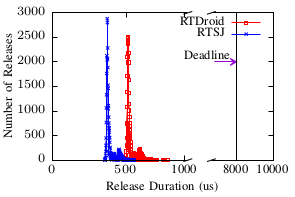
\includegraphics[width=\textwidth]{cochlear}
		\caption{Cochlear Implant}
		\label{fig:cochlear}
	\end{subfigure}
	~ 
	\begin{subfigure}[b]{0.3\textwidth}
		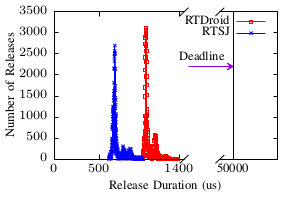
\includegraphics[width=\textwidth]{jpapabench}
		\caption{jPapaBench}
		\label{fig:jpapabench}
	\end{subfigure}
	~
	\begin{subfigure}[b]{0.3\textwidth}
		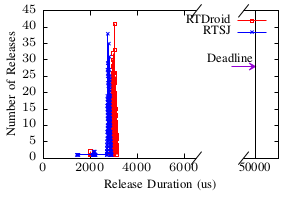
\includegraphics[width=\textwidth]{turbine}
		\caption{Wind Turbine Health Monitoring}
		\label{fig:turbine}
	\end{subfigure}
	\caption{Misurazione delle prestazioni}\label{fig:appperformance}
\end{figure}

Figura~\ref{fig:appperformance} mostra la durata delle esecuzioni per ogni release. I grafici mostrano che l'utilizzo della memoria scoped e la comunicazione attraverso canali real-time aumenta il tempo di esecuzione di ogni release, ma con un overhead limitato. Android, al contrario, è tutto fuori che prevedibile, come mostrato in Figura~\ref{fig:performancenx5}. Infatti la varianza nella durata è altissima. 

\begin{figure}[h]
	\centering
	\begin{subfigure}[b]{0.45\textwidth}
		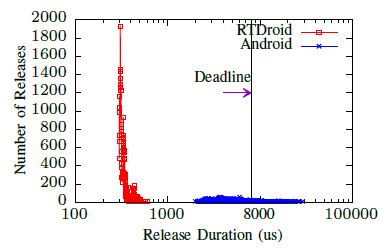
\includegraphics[width=\textwidth]{cochlearAudioproc}
		\caption{Cochlear Implant: Durata dell'elaborazione audio}
		\label{fig:cochlearAudioproc}
	\end{subfigure}
	~ 
	\begin{subfigure}[b]{0.45\textwidth}
		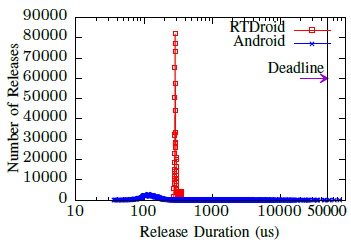
\includegraphics[width=\textwidth]{jpapabenchStabilization}
		\caption{jPapaBench: Durata della stabilizzazione}
		\label{fig:jpapabenchStabilization}
	\end{subfigure}
	\caption{Prestazioni su un Nexus5}\label{fig:performancenx5}
\end{figure}

Figura~\ref{fig:statduratabench} quantifica i risultati delle precedenti figure. Come già visto, sia RTDroid che RTSJ aggiungono overhead nelle esecuzioni. In jPapaBench RTDroid si comporta peggio di RTSJ. Quest'ultima esegue la stabilizzazione semplicemente leggendo i dati dei sensori da un buffer condiviso, li elabora ed esegue controlli basati sempre sul buffer condiviso. RTDroid, al contrario, utilizza i canali di comunicazione descritti sopra al posto di buffer condivisi, e quindi incorre in un maggiore overhead. Si nota comunque che Android è molto più veloce ad eseguire i compiti, ma ha un'alta percentuale di deadline mancate, inaccettabile in un sistema real-time.
\begin{figure}[h]
	\centering
	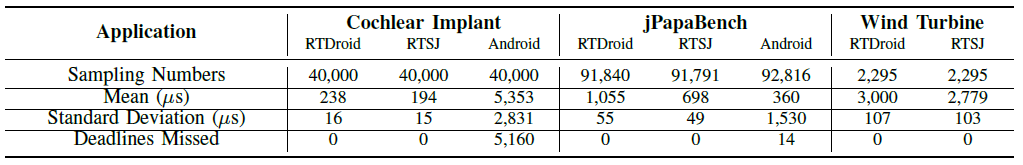
\includegraphics[width=1\linewidth]{statDurataBench}
	\caption{Statistiche della durata delle esecuzioni}
	\label{fig:statduratabench}
\end{figure}

Figura~\ref{fig:cdfappperformance} mostra i CDF degli esperimenti condotti. Le curve di RTSJ e di RTDroid sono simili. Basandoci su questi dati, e sui dati di Figura~\ref{fig:statduratabench} si può concludere che RTDroid aggiunge latenza, ma che questa non ha un impatto significativo sulla prevedibilità delle applicazioni che vengono eseguite. Ancora una volta, questo overhead è dovuto al paradigma di comunicazione utilizzato. 

\begin{figure}[h]
	\centering
	\begin{subfigure}[b]{0.3\textwidth}
		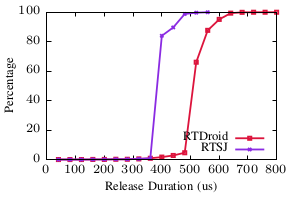
\includegraphics[width=\textwidth]{cochlearCDF}
		\caption{CDF per Cochlear Implant}
		\label{fig:cochlearcdf}
	\end{subfigure}
	~ 
	\begin{subfigure}[b]{0.3\textwidth}
		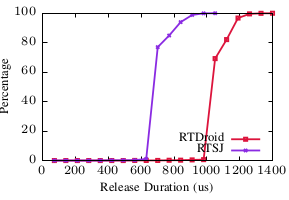
\includegraphics[width=\textwidth]{jpapabenchCDF}
		\caption{CDF per jPapaBench}
		\label{fig:jpapabenchcdf}
	\end{subfigure}
	~
	\begin{subfigure}[b]{0.3\textwidth}
		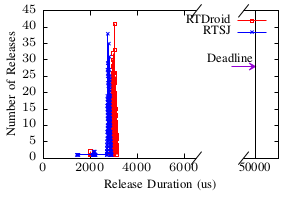
\includegraphics[width=\textwidth]{turbine}
		\caption{CDF per Wind Turbine Health MonitoringCDF}
		\label{fig:turbinecdf}
	\end{subfigure}
	\caption{CDF per la misurazione delle prestazioni}\label{fig:cdfappperformance}
\end{figure}

Figura~\ref{fig:cdfaudionx5} e Figura~\ref{fig:cdfstabnx5} mostrano i CDF del confronto con Android. Non sorprendentemente si nota che una porzione non banale di release in Android incorre in ritardi significativi, anche quando il sistema non è sovraccarico. Sebbene RTDroid aggiunga un overhead rispetto a RTSJ, il beneficio rispetto ad Android è enorme. La complessità delle operazioni sottostanti (gestione della memoria scoped) è nascosta dal design, e il sistema disaccoppia configurazione dei task real-time (manifest) dalla logica dell'applicazione (codice Java). Inoltre semplifica la comunicazione attraverso diversi tipi di canali in pieno stile Android. Figura~\ref{fig:codecomplx} mostra delle tipiche misure di complessità del codice scritto per le tre piattaforme analizzate, escludendo le librerie esterne utilizzate. Applicazioni scritte per RTDroid sono composte da meno linee di codice. RTSJ, infatti, richiede che i programmatori facciano tutto a mano: creazione dei task e rilascio a multi-threading. In RTDroid tutta la complessità è nascosta e i componenti sono dichiarati nel manifest, in modo che il sistema possa gestirli in automatico sulla base della configurazione fornita. Inoltre, dato che è previsto un paradigma di comunicazione esplicito, non è necessario che i programmatori scrivano codice per la sincronizzazione della comunicazione, riducendo il rischio di errori.

\begin{figure}[h]
	\centering
	\begin{subfigure}[b]{0.45\textwidth}
		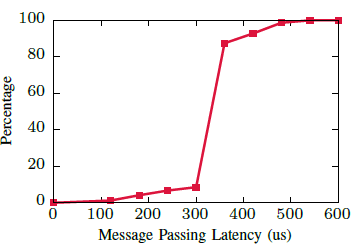
\includegraphics[width=\textwidth]{audioprocRTDroid}
		\caption{Durata dell'elaborazione audio su RTDroid}
		\label{fig:cochlearAudioprocRT}
	\end{subfigure}
	~ 
	\begin{subfigure}[b]{0.45\textwidth}
		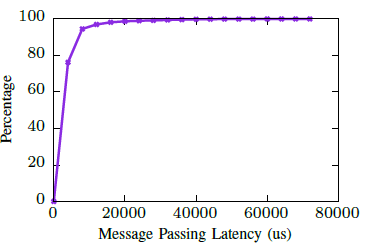
\includegraphics[width=\textwidth]{audioprocAndroid}
		\caption{Durata dell'elaborazione audio su Android}
		\label{fig:cochlearAudioprocAN}
	\end{subfigure}
	\caption{CDF per l'elaborazione audio su un Nexus5}\label{fig:cdfaudionx5}
\end{figure}

\begin{figure}[h]
	\centering
	\begin{subfigure}[b]{0.45\textwidth}
		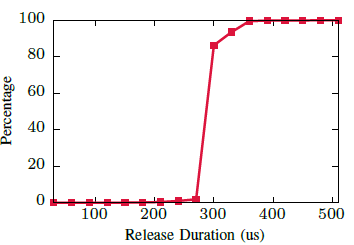
\includegraphics[width=\textwidth]{stabilizationRTDroid}
		\caption{Durata della stabilizzazione su RTDroid}
		\label{fig:stabilizationRTDroid}
	\end{subfigure}
	~ 
	\begin{subfigure}[b]{0.45\textwidth}
		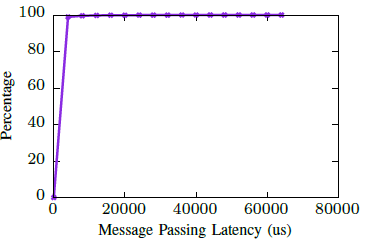
\includegraphics[width=\textwidth]{stabilizationAndroid}
		\caption{Durata della stabilizzazione su Android}
		\label{fig:stabilizationAndroid}
	\end{subfigure}
	\caption{CDF per la stabilizzazione su un Nexus5}\label{fig:cdfstabnx5}
\end{figure}

\begin{figure}[h]
	\centering
	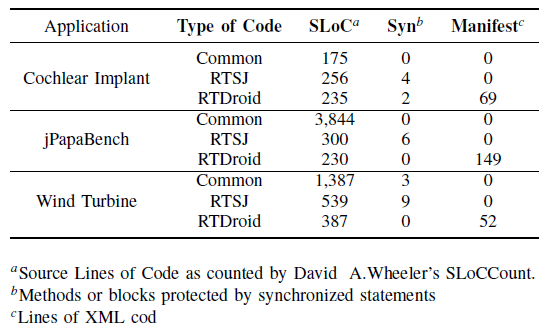
\includegraphics[width=0.7\linewidth]{codecomplx}
	\caption{Complessità del codice}
	\label{fig:codecomplx}
\end{figure}
